\documentclass{article}
\usepackage[utf8]{inputenc}
\usepackage[italian]{babel}
\usepackage{graphicx}
\usepackage{fancyhdr}
\usepackage{lastpage}
\usepackage{hyperref}
\hypersetup{
	colorlinks,
	citecolor=black,
	filecolor=black,
	linkcolor=black,
	urlcolor=blue
}

% Header e footer
\pagestyle{fancy}
\fancyhf{}
\fancyhead[L]{Sushi Nakamura}
\fancyhead[R]{\leftmark}
\fancyfoot[R]{pagina \thepage\ di \pageref{LastPage}}
\renewcommand{\headrulewidth}{1pt}
\renewcommand{\footrulewidth}{1pt}

\begin{document}
	% Frontespizio
	\begin{titlepage}
		\begin{figure}[http]
			\centering
			
\includegraphics[width=6cm]{logo.jpg}
		\end{figure}
	
		\vspace*{2cm}
		
		{\huge\bfseries\centerline{Sushi Nakamura} }
		\centerline{Progetto di Tecnologie Web A.A. 2019/2020}
		
		\vspace*{1cm}
		{\bfseries \centerline{Informazioni sul gruppo}}
		\begin{center}
			\begin{tabular}{ c|l } 
				Membri & Dindinelli Alessandro - 1170457\\ 
				& Frison Nicolò - 1147682\\ 
				& Giardina Mirco - 1136663\\
				& Tommasin Alessandro - 1189293\\ 
			\end{tabular}
		\end{center}
		
		\vspace*{\fill}
		
	\end{titlepage}
	
	% Pagina indici
	\clearpage
	\renewcommand*\contentsname{Indice}
	\tableofcontents	
	\newpage
	
	% Contenuto
	\section{Introduzione}
		\subsection{Abstract}
			Il sito web \textbf{Sushi Nakamura} è stato sviluppato per permettere all'omonimo ristorante di Padova un mezzo per promuovere sè stesso ed il suo nuovo servizio di take away.
			Nel sito è possibile reperire tutte le informazioni riguardanti i contatti ed i prodotti che possono essere acquistati.
			Inoltre l'amministratore ha la possibilità di inserire, rimuovere e modificare eventuali articoli in vendita e news che possono essere visualizzate dagli utenti.
	\section{Analisi}
		\subsection{Analisi dell'utenza}
			Questo sito possiede un bacino di utenza variegato in quanto si è ritenuto possibile che sia utenti molto giovani che utenti in età più adulta possano essere interessati ad accedere al sito e ai suoi servizi.
			La parte più giovane molto probababilmente è abituata all'utilizzo di servizi di take away da dispositivi mobile e probabilmente sfrutterà la parte del sito adibita all'esposizione dei prodotti disponibili e all'ordinazione take away.
			La controparte adulta, invece, probabilmente sfrutterà di più il sito per consultare sia i prodotti disponibili che per trovare le informazioni riguardanti l'ubicazione del ristorante ed eventualmente il contatto telefonico per prenotare. 
		\subsection{Conclusione}
			Il sito dovrà quindi essere fornito di una sezione che permetta agli utenti di trovare i prodotti divisi in categorie. Dovrà inoltre gestire l'ordinazione, il pagamento e l'eventuale spedizione del prodotto, nel caso in cui si selezioni la spedizione a domicilio.
			Si ritiene possa essere un'aggiunta interessante avere la possibilità di salvare i metodi di pagamento e di spedizione in modo tale da non doverli reinserire ad ogni acquisto (nel caso di utente autenticato).	
	\section{Progettazione}
		\subsection{Obiettivi}
		    Gli obiettivi principali perseguiti durante la progettazione del sito sono i seguenti:
		    \begin{itemize}
		        \item \textbf{Separazione tra struttura, presentazione e comportamento:}
		        Obiettivo fondamentale, in quanto raggiungerlo permette di soddisfare più agevolmente anche gli altri punti. 
		        La struttura è stata realizzata con documenti in XHTML 1.0 Strict dove possibile, così da garantire una maggiore retrocompatibilità con vecchi browsers, ed HTML5 dove si sono ritenute necessarie le funzionalità aggiuntive permesse dal linguaggio. 
		        La presentazione è stata sviluppata con fogli di stile CSS linkati, mentre il comportamento con script esterni realizzati in Javascript e PHP. In questo modo la struttura non dovrà cambiare, anche a seguito di modifiche alla presentazione del sito.
		        Tutto il codice redatto è stato scritto secondo le raccomandazioni W3C, accertando poi che siano state rispettate, validando HTML e CSS con i rispettivi tool di W3C.
		        \item \textbf{Accessibilità:}
		        Il sito deve poter essere fruibile agevolmente dal maggior numero di utenti possibile, compresi quelli con differenti tipi di disabilità. Per garantire una buona accessibilità, alcune misure adottate sono:
		        \begin{itemize}
		            \item Uso dei tabindex nel menù di navigazione;
		            \item Testo alternativo per le immagini;
		            \item Assenza di link circolari;
		            \item Testi e link con buoni livelli di contrasto;
		            \item Uso dell'attributo lang per testi non in italiano;
		        \end{itemize}
		        \item \textbf{Fluidità:}
		        Il sito deve poter essere consultabile tramite varie tipologie di dispositivi, tra cui PC desktop, tablet e smartphone. Bisogna quindi garantire una buona adattabilità alle differenti dimensioni di schermo.
		        \item \textbf{Fruibilità:}
		        Per realizzare un sito navigabile intuitivamente si sono seguite alcune linee guida comuni nel web, come ad esempio:
		        \begin{itemize}
		            \item Sfruttare un layout ben strutturato, che faciliti l'individuazione del contenuto di interesse;
		            \item Agevolare lo scroll tramite link relativi per raggiungere diversi punti di una stessa pagina;
		            \item Mantenere colorazioni diverse per link visitati e non;
		        \end{itemize}
		    \end{itemize}
		\subsection{Layout}
			Si è deciso di strutturare il sito con un layout a colonna singola, come illustrato in Figura 1. Questo modello permette una buona mantenibilità, dato che anche in caso si effettuino modifiche al contenuto della pagina la sua presentazione rimane uniforme, avendo a disposizione l'intera larghezza della finestra. 
		    Dimostra di essere anche un layout molto flessibile in quanto la transizione dalla presentazione su desktop a quella su dispositivi mobili risulta fluida.
		    \begin{figure}[http] %Verificare posizione immagine dopo aver scritto i capitoli precedenti;
		        \centering
		        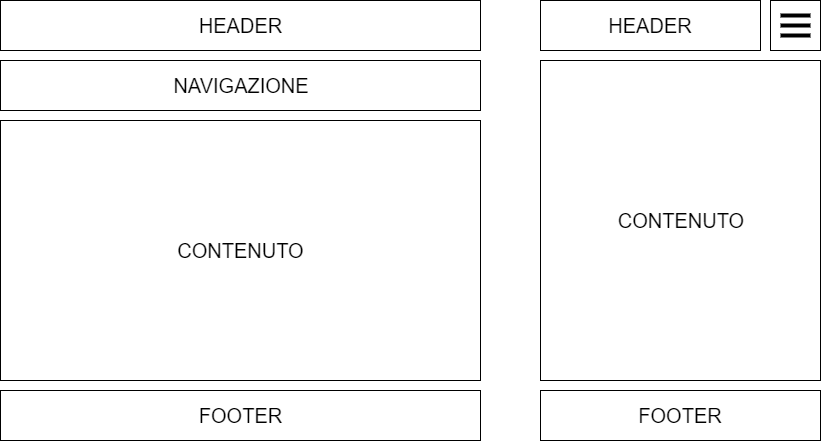
\includegraphics[width=\textwidth]{schema_layout.png}
		        \caption{Schema del layout per desktop e mobile.}
		        \label{fig:layout}
		    \end{figure}
		    \bigbreak
		    L'Header, che contiene logo e nome del ristorante, fondamentalmente varia solo in dimensione nella transizione tra i due layout.
		    \bigbreak
		    Il Footer invece contiene informazioni generali sul ristorante, la dichiarazione del Copyright, e l'eventuale immagine di certificata validazione delle pagine XHTML 1.0 Strict. Per garantire una lettura migliore, restringendo la finestra si passa ad una visualizzazione da doppia a singola colonna.
		    \bigbreak
		    La principale differenza tra i layout scelti sta nella posizione e presentazione del menù di navigazione. 
		    \newline Nei device con finestre di visualizzazione sufficentemente larghe si è scelto di disporre le voci del menù in riga, creando quindi una barra di navigazione. I link alle varie pagine principali del sito sono disposte a partire da sinistra, mentre quelli riguardanti pagine per gli utenti e le operazioni a loro disposizione si trovano a partire da destra.
		    \newline Nei dispositivi più piccoli si è deciso invece di creare un menù espandibile, raggiungibile premendo sull'icona ad hamburger nell'angolo in alto a destra, che mostra tutte le voci disponibili, per rispettare il comportamento più comune che un utente medio si aspetta utilizzando uno smartphone.
		\subsection{Accessibilità}
	\section{Implementazione}
		\subsection{Linguaggi}
			\subsubsection{XHTML 1.0 Strict e HTML5}
			    Come già detto, per la realizzazione del sito si è optato per avere sia pagine in XHTML 1.0 Strict, che in HTML5. L'uso di XHTML 1.0 garantisce una migliore retrocompatibilità con browsers più datati ed una migliore aderenza del codice agli standard di correttezza, ma HTML5 permette di sfruttare alcune funzionalità aggiuntive che abbiamo sfruttato ad esempio in vari form per inserire input di tipo \textit{date}, utilizzare \textit{placeholder} o per rendere dei campi \textit{required} in modo da chiarire e migliorare l'usabilità del sito. In entrambi i casi per ottenere codice pulito si sono seguiti i seguenti principi:
			    \begin{itemize}
			        \item Mantenere la separazione tra struttura e presentazione, usando file separati linkati nell'header;
			        \item Ogni $<$tag$>$ aperto deve essere poi chiuso $<$/tag$>$ (oppure $<$tag /$>$);
			        \item I tag di intestazione vanno usati in base all'importanza di ciò che racchiudono, e non in base all'estetica base html;
			    \end{itemize}
			    \newline In generale, per garantire un codice corretto, sono state seguite le linee guida che sono state illustrate durante il corso di Tecnologie Web e quelle dello standard W3C. La verifica del codice è stata poi effettuata  utilizzando il tool di validazione W3C Validator%
			    \footnote{Riferimento al sito di W3C Validator \url{https://validator.w3.org/}},
			    la piattaforma SonarCloud% 
			    \footnote{Riferimento al sito di SonarCloud \url{https://sonarcloud.io/about}}
			    integrata con GitHub
			    ed il software di validazione di siti Total Validator.%
			    \footnote{Riferimento al sito di Total Validator \url{https://www.totalvalidator.com/}}
			    \newline Si è prestata attenzione al ruolo dei metatag nell'header, il cui buon uso migliora anche l'indicizzazione del sito da parte dei motori di ricerca, aspetto fondamentale per un'attività commerciale che voglia ricevere un'adeguata visibilità nel web.
			    \newline Si è deciso di fare uso anche di tabelle, rendendole più agevolmente accessibili tramite l'uso di adeguati \textit{summary}, e di \textit{scope} su colonne e righe di interesse.
			\subsubsection{CSS}
				CSS è stato usato per la presentazione grafica delle pagine HTML. Si è cercato di puntare ad un discreto riutilizzo del codice creando classi da poter usare su più pagine, come per esempio bottoni e form preimpostati, che poi potevano venire personalizzati dove necessario sovrascrivendo le regole necessarie. Il contenuto di ogni pagina è identificato da una classe così da avere una formattazione del testo omogenea mentre per impaginare le pagine specifiche si è optato per un identificativo univoco per ogni pagina.
			\subsubsection{PHP}
			\subsubsection{SQL}
			Sql è stato usato per codificare il database. Si rimanda al file \textit{creazione\_database.sql} nella cartella \textit{Database} [\href{https://github.com/Mirco469/ProgettoSushi/tree/master/Database}{url}] della repository per il file di costruzione del database. Di seguito il diagramma ER del database:\newline
			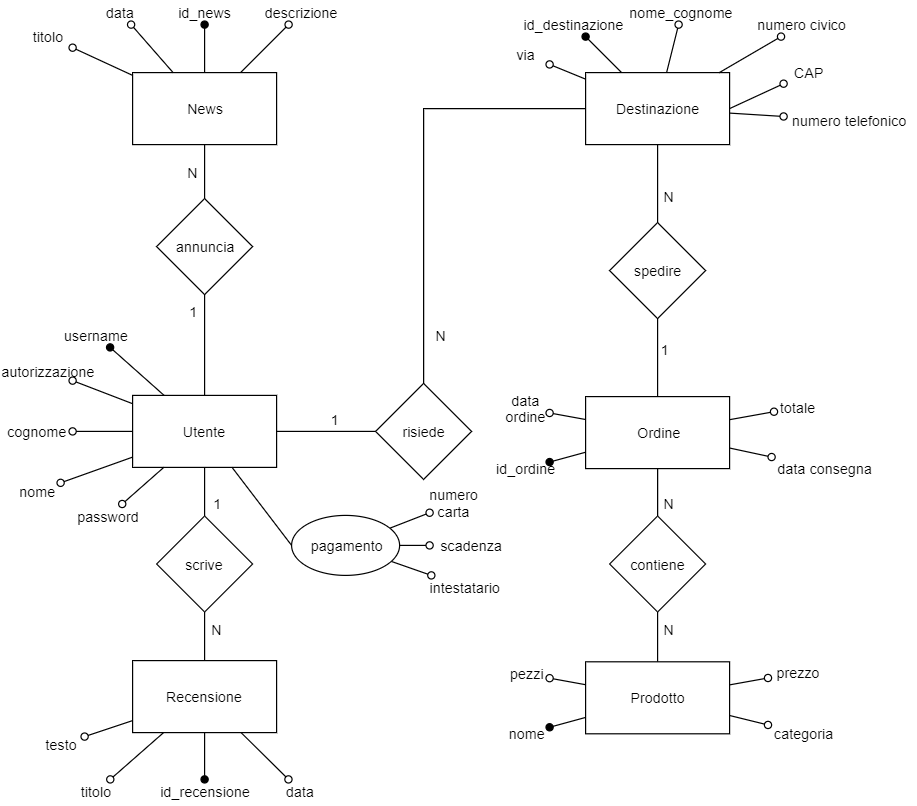
\includegraphics[width=12cm]{DiagrammaER.png}
			\subsubsection{JavaScript}
	\section{Fase di test}
		\subsection{Strumenti usati}
			\subsubsection{W3C HTML Validator}
				Le pagine html sono state validate usando il validatore fornito dall'organizazione W3C per garantire la corretta visualizzazione del contenuto della pagina senza fare entrare i browser in {\bfseries Quirks Mode}. \'E stato usato anche per validare il risultato delle pagine php incollando il sorgente ottenuto facendo eseguire lo script php.
			\subsubsection{W3C CSS Validator}
				Tutti i file CSS sono stati validati usando lo strumento di validazione fornito da W3C per assicurarsi che fossero strutturati correttamente.
			\subsubsection{TotalValidator}
			    Con questo strumento abbiamo validato tutto il codice HTML. Principalmente errori segnalati dal programma riguardano direttive sull'uso delle regole WAI-ARIA% 
			    \footnote{Web Accessibility Initiative - Accessible Rich Internet Applications -  \url{https://www.w3.org/WAI/standards-guidelines/aria/}}
			    relative all'utilizzo delle \textit{aria-label}, cosa che non è necessaria in questo caso, in quanto i vari link e buttons sono facilmente indiduabili ed interpretabili.
			\subsubsection{SonarCloud}
				Servizio integrato con GitHub per la verifica del codice nella repository. Ad ogni push veniva fatta un {\bfseries analisi statica} del codice alla ricerca di problemi e vulnerabilità come ad esempio un problema comune è stata la ripetizione rindondate di regole css. Questa fase di test era bloccante, ovvero perchè il codice venisse aggiunto dovevano prima essere risolti i problemi.
	\section{Organizzazione del lavoro}
		Il progetto è stato suddiviso in modo tale che ogni membro avesse la possibilità di creare sia alcune pagine HTML che il relativo CSS, facendo da verificatore nelle pagine degli altri membri.
		Lo stesso può essere detto per quanto concerne PHP, JavaScript e la creazione ed il popolamento del database.
		La sviluppo può essere seguito nella repossitory di GitHub utilizzata:
		\newline
		\newline
		\centerline{ \url{https://github.com/Mirco469/ProgettoSushi}}

\end{document}
